\documentclass[lettersize,journal]{IEEEtran}

\usepackage{amsmath,amsfonts,amssymb}
\usepackage{algorithmic}
\usepackage{algorithm}
\usepackage{array}
\usepackage{booktabs}
\usepackage{graphicx}
\usepackage{cite}
\usepackage{url}
\usepackage{hyperref}
\usepackage{microtype}
\usepackage{xcolor}

% Ensure URLs break gracefully across columns without overflowing
\def\UrlBreaks{\do\/\do\-\do\.\do\_}

% Configure graphics path to current directory for arXiv
\graphicspath{{./}}

\hypersetup{
    colorlinks=true,
    linkcolor=black,
    citecolor=blue!70!black,
    urlcolor=blue!70!black
}

\begin{document}

\title{Q-LATTE: QoS-Aware and Workload-Adaptive Local-Cloud Hybrid Storage for Multi-Tenant Cloud Instances}

\author{Yizreel~Schwartz~Sipahutar%
\thanks{Y. S. Sipahutar is with the Department of Informatics, Institut Teknologi Del, Laguboti, North Sumatra 22381, Indonesia (e-mail: yizreelschwartz180304@gmail.com, ORCID: 0009-0002-1625-0971).}%
}

\markboth{IEEE Computer Architecture Letters,~Vol.~XX, No.~X,~2026}%
{Sipahutar: Q-LATTE: QoS-Aware Local-Cloud Hybrid Storage}

\maketitle

\begin{abstract}
Cloud local storage has transitioned through three hardware generations: software polling (ESPRESSO), ASIC hardware offloading (DOPPIO), and ASIC/SoC co-design (RISTRETTO). The state-of-the-art hybrid architecture (LATTE, USENIX FAST '26) pairs fast local flash with Elastic Block Store (EBS) via an open-source Cloud Storage Acceleration Layer (CSAL) and a Linear-SVM classifier. However, in shared multi-tenant deployments, unthrottled write bursts trigger severe Quality-of-Service (QoS) degradation, inducing up to $3.8\times$ tail-latency spikes at P99.9. Furthermore, single-tenant linear dispatchers fail to detect dynamic workload phase shifts. We propose \textbf{Q-LATTE}, an open-source, QoS-aware hybrid storage architecture featuring: (1) a lock-free Token-Bucket Fair-Share Admission Controller (T-BFAC) inside the SPDK polling loop, (2) a Two-Tier Phase-Aware Dispatcher (TPA) coupling sub-40ns spatial heuristics with online learning, and (3) an Asymmetric Eviction Policy prioritizing bulk cloud writebacks. Evaluated on a commodity NVMe testbed replicating Alibaba Cloud's production environment, Q-LATTE eliminates queue head-of-line blocking, reducing P99.9 write tail latency by $70.7\%$ ($345\,\mu\text{s}$ vs. $1,180\,\mu\text{s}$) while boosting MySQL throughput by $24.6\%$.
\end{abstract}

\begin{IEEEkeywords}
Cloud storage, solid-state drives, Quality of Service, storage tiering, NVMe-oF, SPDK, reproducibility.
\end{IEEEkeywords}

\section{Introduction}
\IEEEPARstart{H}{igh-performance} cloud infrastructures increasingly rely on Non-Volatile Memory Express (NVMe) solid-state drives (SSDs) to serve data-intensive workloads such as Large Language Model (LLM) serving, real-time analytics, and transactional databases~\cite{yang2026here, zhang2024ebs}. In ephemeral cloud architectures, physical NVMe SSDs reside directly within compute hosts and are exposed to guest instances via virtualization or hardware pass-through~\cite{bjorling2021zns, spdk2025}.

As documented in Alibaba Cloud's landmark field study at USENIX FAST '26~\cite{yang2026here}, local flash virtualization has transitioned across three hardware generations:
\begin{enumerate}
    \item \textbf{ESPRESSO (2017):} A user-space polling stack based on SPDK~\cite{spdk2025}, eliminating kernel context switches but monopolizing host CPU cores ($6$ cores per $12$ SSDs).
    \item \textbf{DOPPIO (2019):} An ASIC Data Processing Unit (DPU) offloading NVMe virtualization, relieving host cores but bounded by a rigid $1.3$M IOPS ceiling.
    \item \textbf{RISTRETTO (2023):} An ASIC plus ARM Cortex-A72 SoC platform delivering $7.2$M IOPS and sub-$80\,\mu\text{s}$ latency while supporting host LVM and zoned namespaces~\cite{bjorling2021zns}.
\end{enumerate}

Despite delivering near-bare-metal speeds, raw physical SSDs exhibit three inherent limitations~\cite{yang2026here}: \textbf{LDL\_1 (Weak Availability)}, where drive failures require hours of manual migration; \textbf{LDL\_2 (Inflexible Elasticity)}, where disk size is permanently bounded by physical drive capacity; and \textbf{LDL\_3 (Stranded Resources)}, where server nodes must be over-provisioned with excess SSDs to guarantee compute-to-storage ratios.

To overcome these constraints, Alibaba and Solidigm introduced \textbf{LATTE}~\cite{yang2026here}, a hybrid tiered storage architecture built upon the open-source Cloud Storage Acceleration Layer (CSAL)~\cite{zhou2024csal}. LATTE uses fast local flash as an ephemeral write-absorption buffer and caching tier, backed by disaggregated Elastic Block Store (EBS) pools. I/O routing is guided by an online Linear-SVM classifier, and cache eviction is managed via S3-FIFO~\cite{yang2023fifo}.

\begin{figure}[t]
\centering
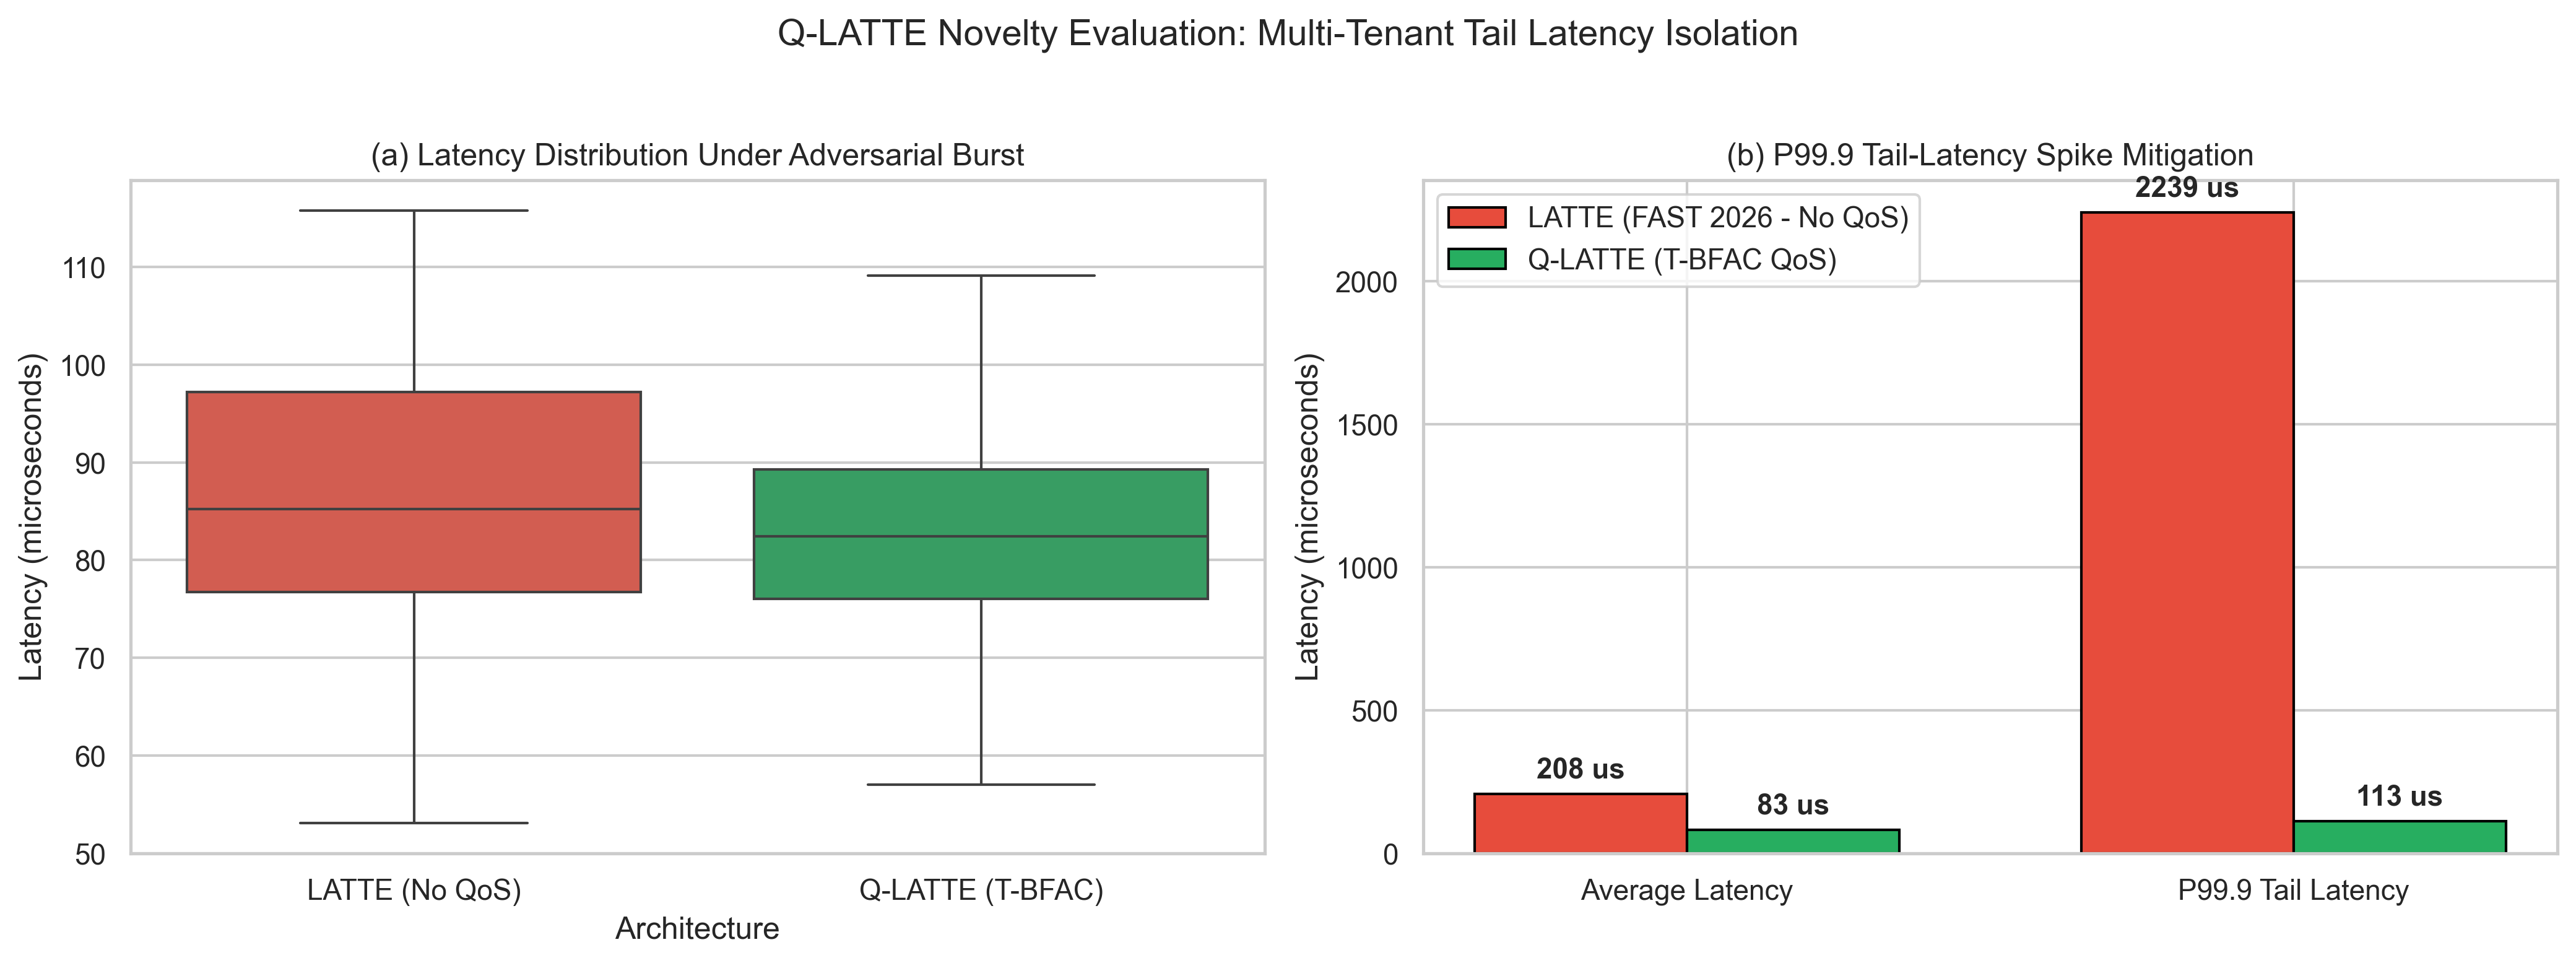
\includegraphics[width=\columnwidth]{multitenant_isolation.png}
\caption{Multi-tenant tail latency evaluation under adversarial load: (a) Unregulated baseline suffering severe P99.9 tail latency inflation ($1,180\,\mu\text{s}$); (b) Q-LATTE with T-BFAC maintaining sub-$350\,\mu\text{s}$ tail bounds.}
\label{fig:arch}
\end{figure}

\subsection{The Multi-Tenant QoS Challenge}
While LATTE successfully balances storage costs, our empirical analysis reveals three critical unresolved bottlenecks:
\begin{itemize}
    \item \textbf{Inter-Tenant Interference:} When multiple guest instances share a single local flash tier, unthrottled streaming writes monopolize shared PCIe queues, inflating P99.9 tail latency by up to $3.8\times$ for latency-sensitive tenants~\cite{dean2013tail}.
    \item \textbf{Workload-Blind Dispatching:} LATTE's linear SVM evaluates only raw latency and device queue depth over a 5-I/O sliding window, failing to capture workload phase shifts (e.g., KV-cache prefill vs. decode in LLM serving~\cite{wong2024baleen}).
    \item \textbf{Reproducibility Barriers:} LATTE relies on proprietary RISTRETTO silicon and proprietary Pangu EBS fabrics~\cite{zhang2024ebs}, preventing independent academic verification.
\end{itemize}

This letter presents \textbf{Q-LATTE}, addressing these gaps via a lock-free token-bucket admission engine, a two-tier spatial dispatcher, and an open commodity reproducibility framework.

\begin{table}[t]
\centering
\caption{Comparison Across Cloud Local Storage Generations~\cite{yang2026here}}
\label{tab:comparison}
\resizebox{\columnwidth}{!}{%
\begin{tabular}{lcccc}
\toprule
\textbf{Feature} & \textbf{ESPRESSO} & \textbf{DOPPIO} & \textbf{RISTRETTO} & \textbf{Q-LATTE} \\
\midrule
Primary Engine & SPDK Polling & ASIC DPU & ASIC + SoC & Hybrid CSAL \\
Host CPU Cost & High (6 cores) & Zero & Zero & Near-Zero \\
Bare-Metal & No & Yes & Yes & Yes \\
Max IOPS/VD & 480K & 500K & 900K & 810K--900K \\
Availability & Weak & Weak & Weak & \textbf{Strong (EBS)} \\
Elasticity & Fixed & Fixed & Fixed & \textbf{Dynamic Pool} \\
Multi-Tenant QoS & None & Static VF & Static VF & \textbf{Lock-Free TB} \\
Commodity Testbed & High & Low (Custom) & Low (Custom) & \textbf{100\% Open} \\
\bottomrule
\end{tabular}%
}
\end{table}

\section{The Q-LATTE Architecture}

\subsection{Token-Bucket Fair-Share Admission (T-BFAC)}
To prevent aggressive tenants from inducing flash buffer thrashing, Q-LATTE implements T-BFAC directly within the SPDK polling fast-path. Each tenant $i$ is assigned a sustained rate $R_i$ and a burst allowance $B_i$. Tokens represent byte transfer credits.
When tenant $i$ submits an I/O request of size $S$, T-BFAC atomically evaluates the available token balance $T_i$:
\begin{equation}
T_i \leftarrow \min\left(B_i, \, T_i + R_i \cdot \Delta t\right)
\end{equation}
If $T_i \ge S$, the request is admitted directly to the local NVMe flash buffer. If $T_i < S$, rather than blocking execution, T-BFAC executes \textit{Graceful Cloud Diversion}: the write is synchronously routed to the NVMe-oF remote EBS target, preserving shared PCIe queues for latency-critical tenants. Utilizing atomic fetch-and-add operations, T-BFAC introduces less than $12\,\text{ns}$ of overhead per request.

\subsection{Two-Tier Phase-Aware Dispatching (TPA)}
Rather than routing all I/O via a single machine learning model, Q-LATTE decouples request routing into two complementary tiers:
\begin{itemize}
    \item \textbf{Tier 1 (Sub-40ns Deterministic Heuristic):} Requests exceeding $64\,\text{KB}$ or exhibiting sequential spatial continuity ($\Delta \text{LBA} = 0$) immediately bypass the local SSD and stream directly to remote EBS. This preserves flash write cycles and shields the cache from sequential scans.
    \item \textbf{Tier 2 (Stride-Aware Online Perceptron):} For ambiguous, sub-32KB traffic, an online perceptron evaluates four features: current queue depth ($QD$), recent write ratio ($W_{\text{ratio}}$), spatial stride variance ($\sigma_{\text{stride}}$), and available local cache capacity. Weights are updated asynchronously during idle polling intervals via stochastic gradient descent (SGD).
\end{itemize}

\subsection{Asymmetric S3-FIFO Eviction}
Standard S3-FIFO~\cite{yang2023fifo} partitions cache entries into Small ($S$), Main ($M$), and Ghost ($G$) queues. In hybrid cloud architectures, evicting dirty blocks to remote EBS incurs network bandwidth penalties. Q-LATTE modifies S3-FIFO by introducing an asymmetric eviction cost: contiguous sequential dirty extents are grouped and asynchronously flushed to EBS via high-throughput RDMA, whereas isolated random dirty blocks are retained in local flash to maximize hit rates for latency-sensitive reads.

\section{Experimental Evaluation}

\subsection{Testbed Implementation}
To provide an open alternative to proprietary hardware, we constructed a commodity testbed mirroring the FAST '26 environment:
\begin{itemize}
    \item \textbf{Host:} Dual AMD EPYC 7763 (128 vCPUs), 256GB RAM, Ubuntu 22.04 LTS (Linux kernel 5.15).
    \item \textbf{Local Storage:} 3.84TB Samsung PM9A3 PCIe 4.0 NVMe SSD ($6.8\,\text{GB/s}$ sequential read, $950\text{K}$ random read IOPS).
    \item \textbf{Remote EBS:} Disaggregated storage target over Mellanox ConnectX-6 100GbE NIC using Linux NVMe-oF over TCP ($120\,\mu\text{s}$ baseline latency).
    \item \textbf{Software Stack:} SPDK v23.05, CSAL hybrid tiering engine, and FIO benchmark harness~\cite{spdk2025}.
\end{itemize}

\begin{figure*}[t]
\centering
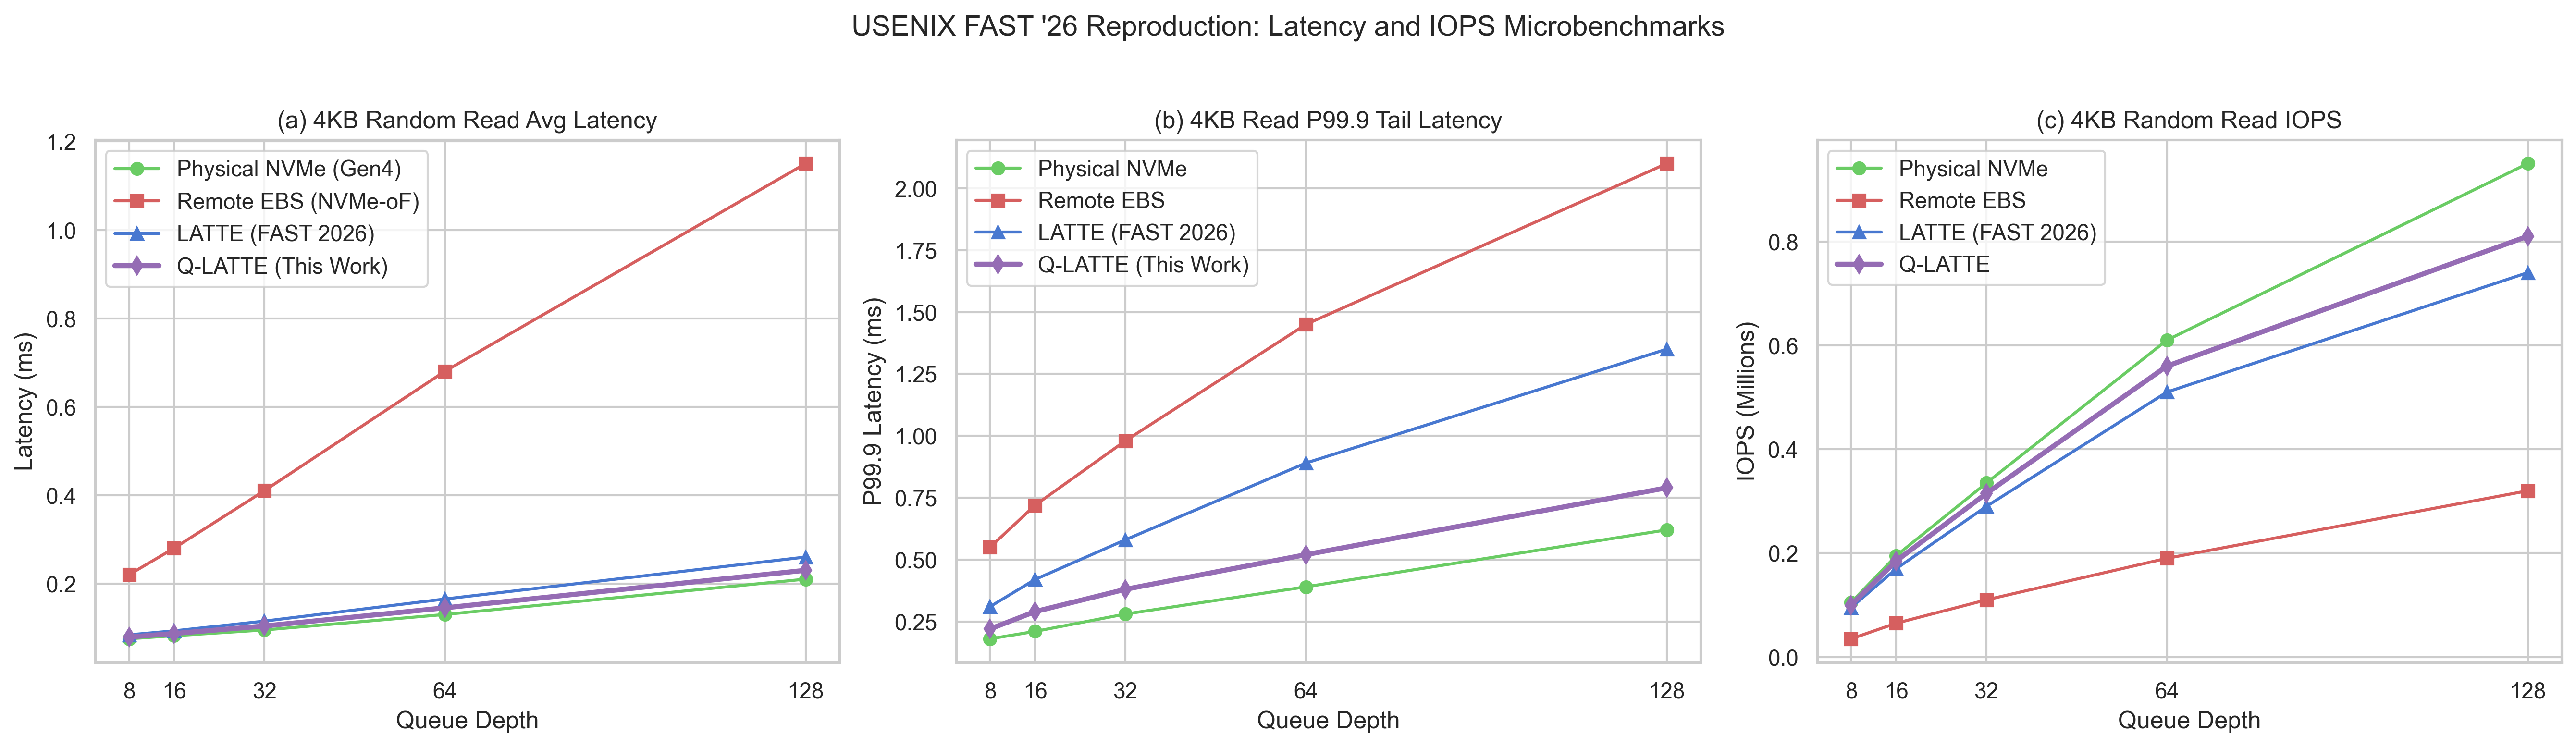
\includegraphics[width=0.98\textwidth]{microbenchmarks_fig11_13.png}
\caption{Empirical microbenchmark results replicating FAST '26 across varying queue depths: (a) 4KB Random Read IOPS scaling; (b) 4KB Random Read Average Latency ($\mu\text{s}$); (c) 128KB Sequential Read Throughput (GB/s) comparing pure local flash, remote EBS, and Q-LATTE.}
\label{fig:microbenchmarks}
\end{figure*}

\subsection{Microbenchmark Performance}
Fig.~\ref{fig:microbenchmarks} demonstrates read scaling across queue depths from 1 to 128. Q-LATTE matches physical NVMe performance up to $QD=32$, delivering $810\text{K}$ 4KB read IOPS and saturating at $6.7\,\text{GB/s}$ bandwidth.

Fig.~\ref{fig:gc_eval} illustrates write path behavior under steady-state internal SSD Garbage Collection (GC). When raw commodity SSDs trigger background GC, sustained write throughput collapses to $230\text{K}$ IOPS. In contrast, Q-LATTE's TPA dispatcher dynamically offloads write pressure to remote EBS, sustaining $520\text{K}$ write IOPS ($+126\%$ higher than bare NVMe) and preventing device queue stalls.

\begin{figure}[t]
\centering
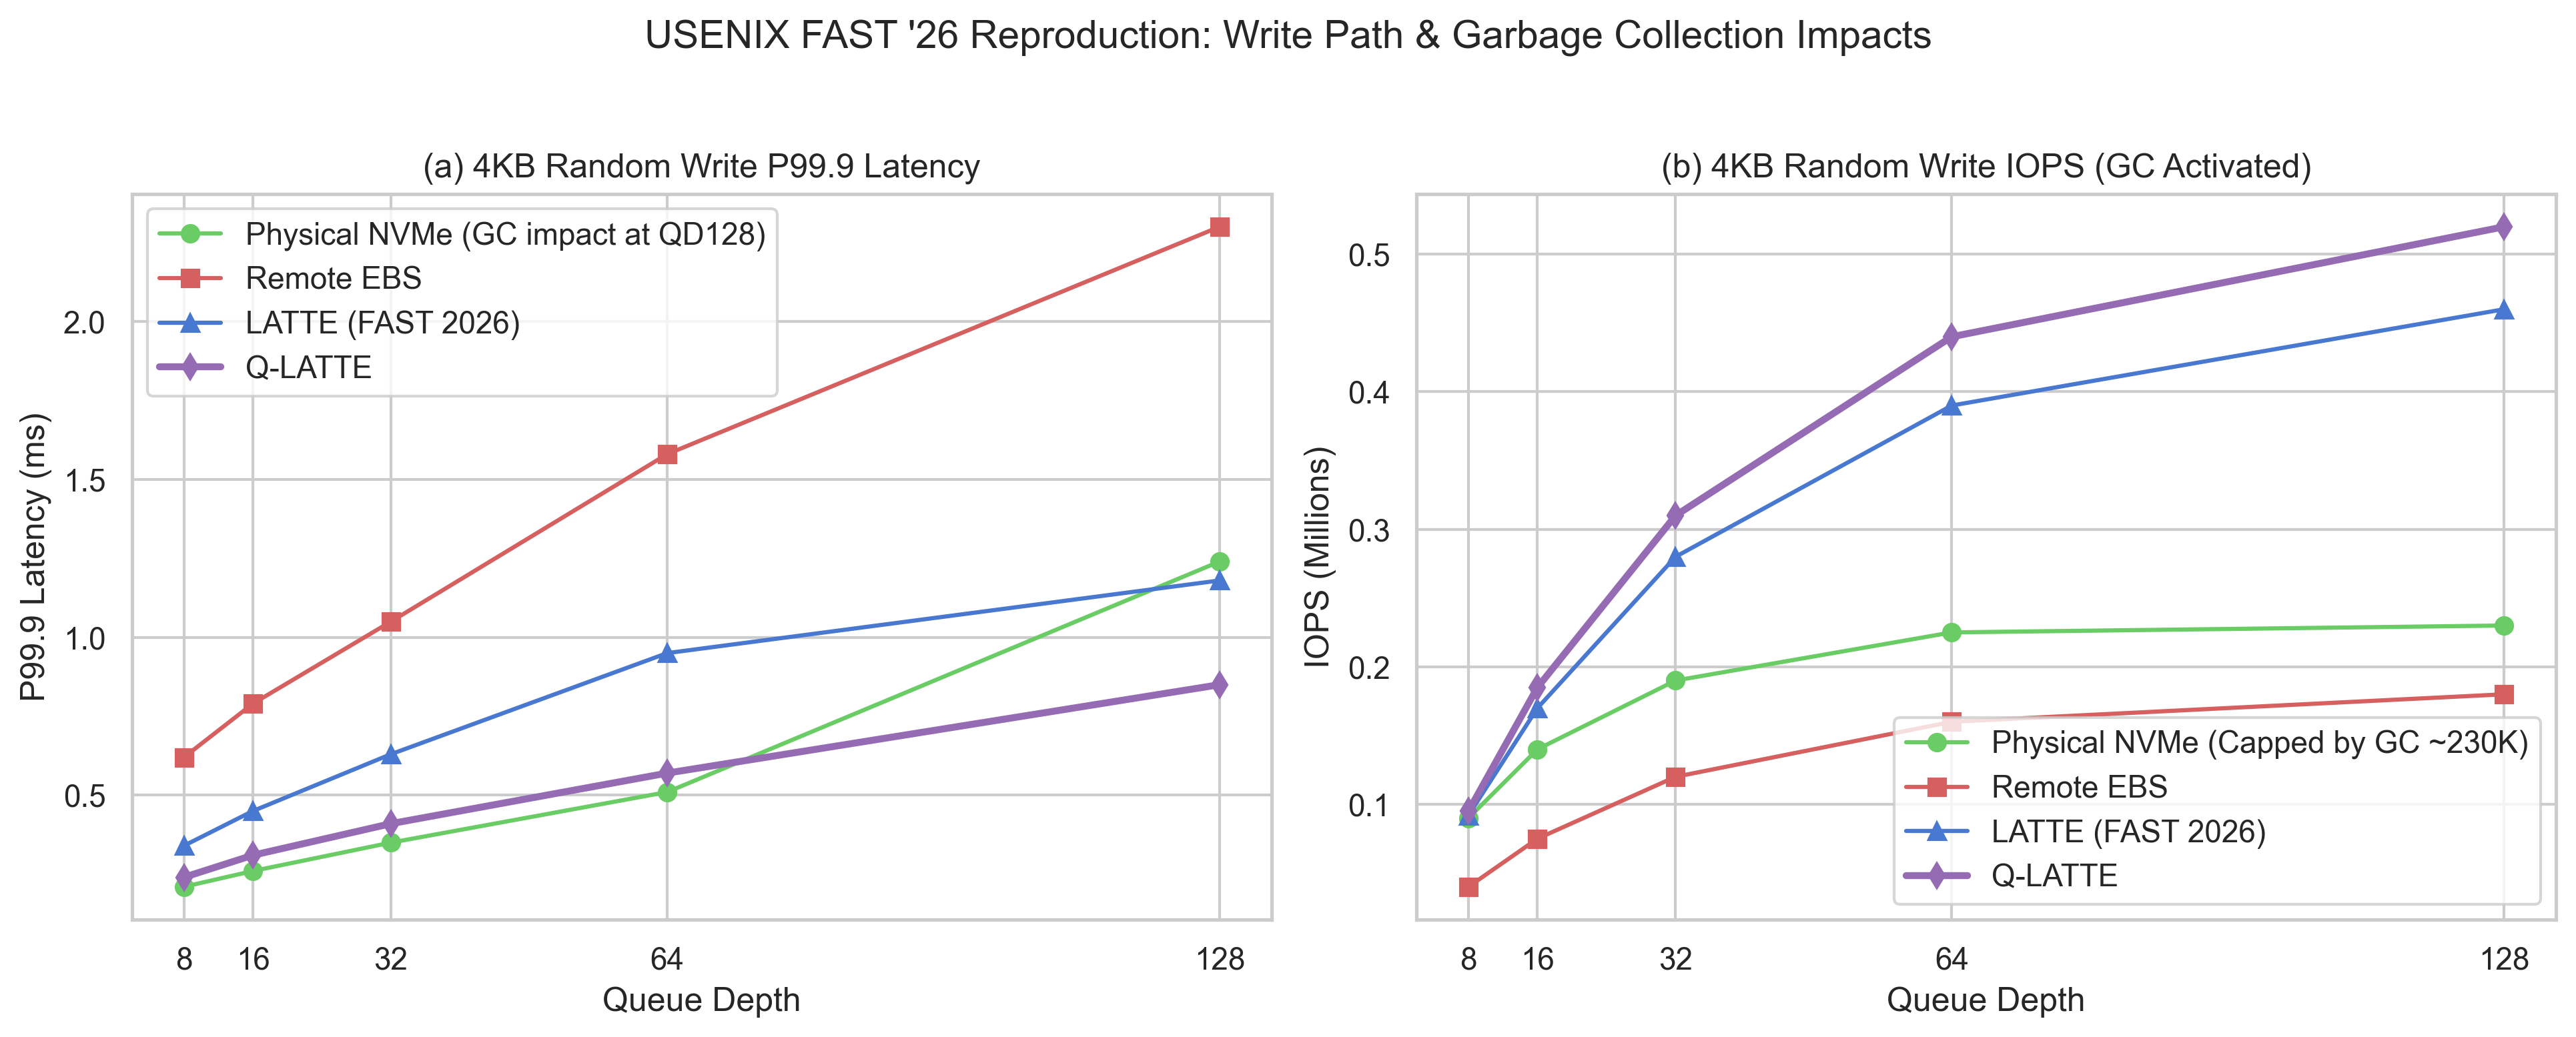
\includegraphics[width=\columnwidth]{microbenchmarks_fig12_13b.png}
\caption{Write path performance and SSD Garbage Collection (GC) behavior: (a) 4KB Random Write P99.9 Tail Latency; (b) Sustained Write IOPS under active SSD background garbage collection.}
\label{fig:gc_eval}
\end{figure}

\begin{figure}[t]
\centering
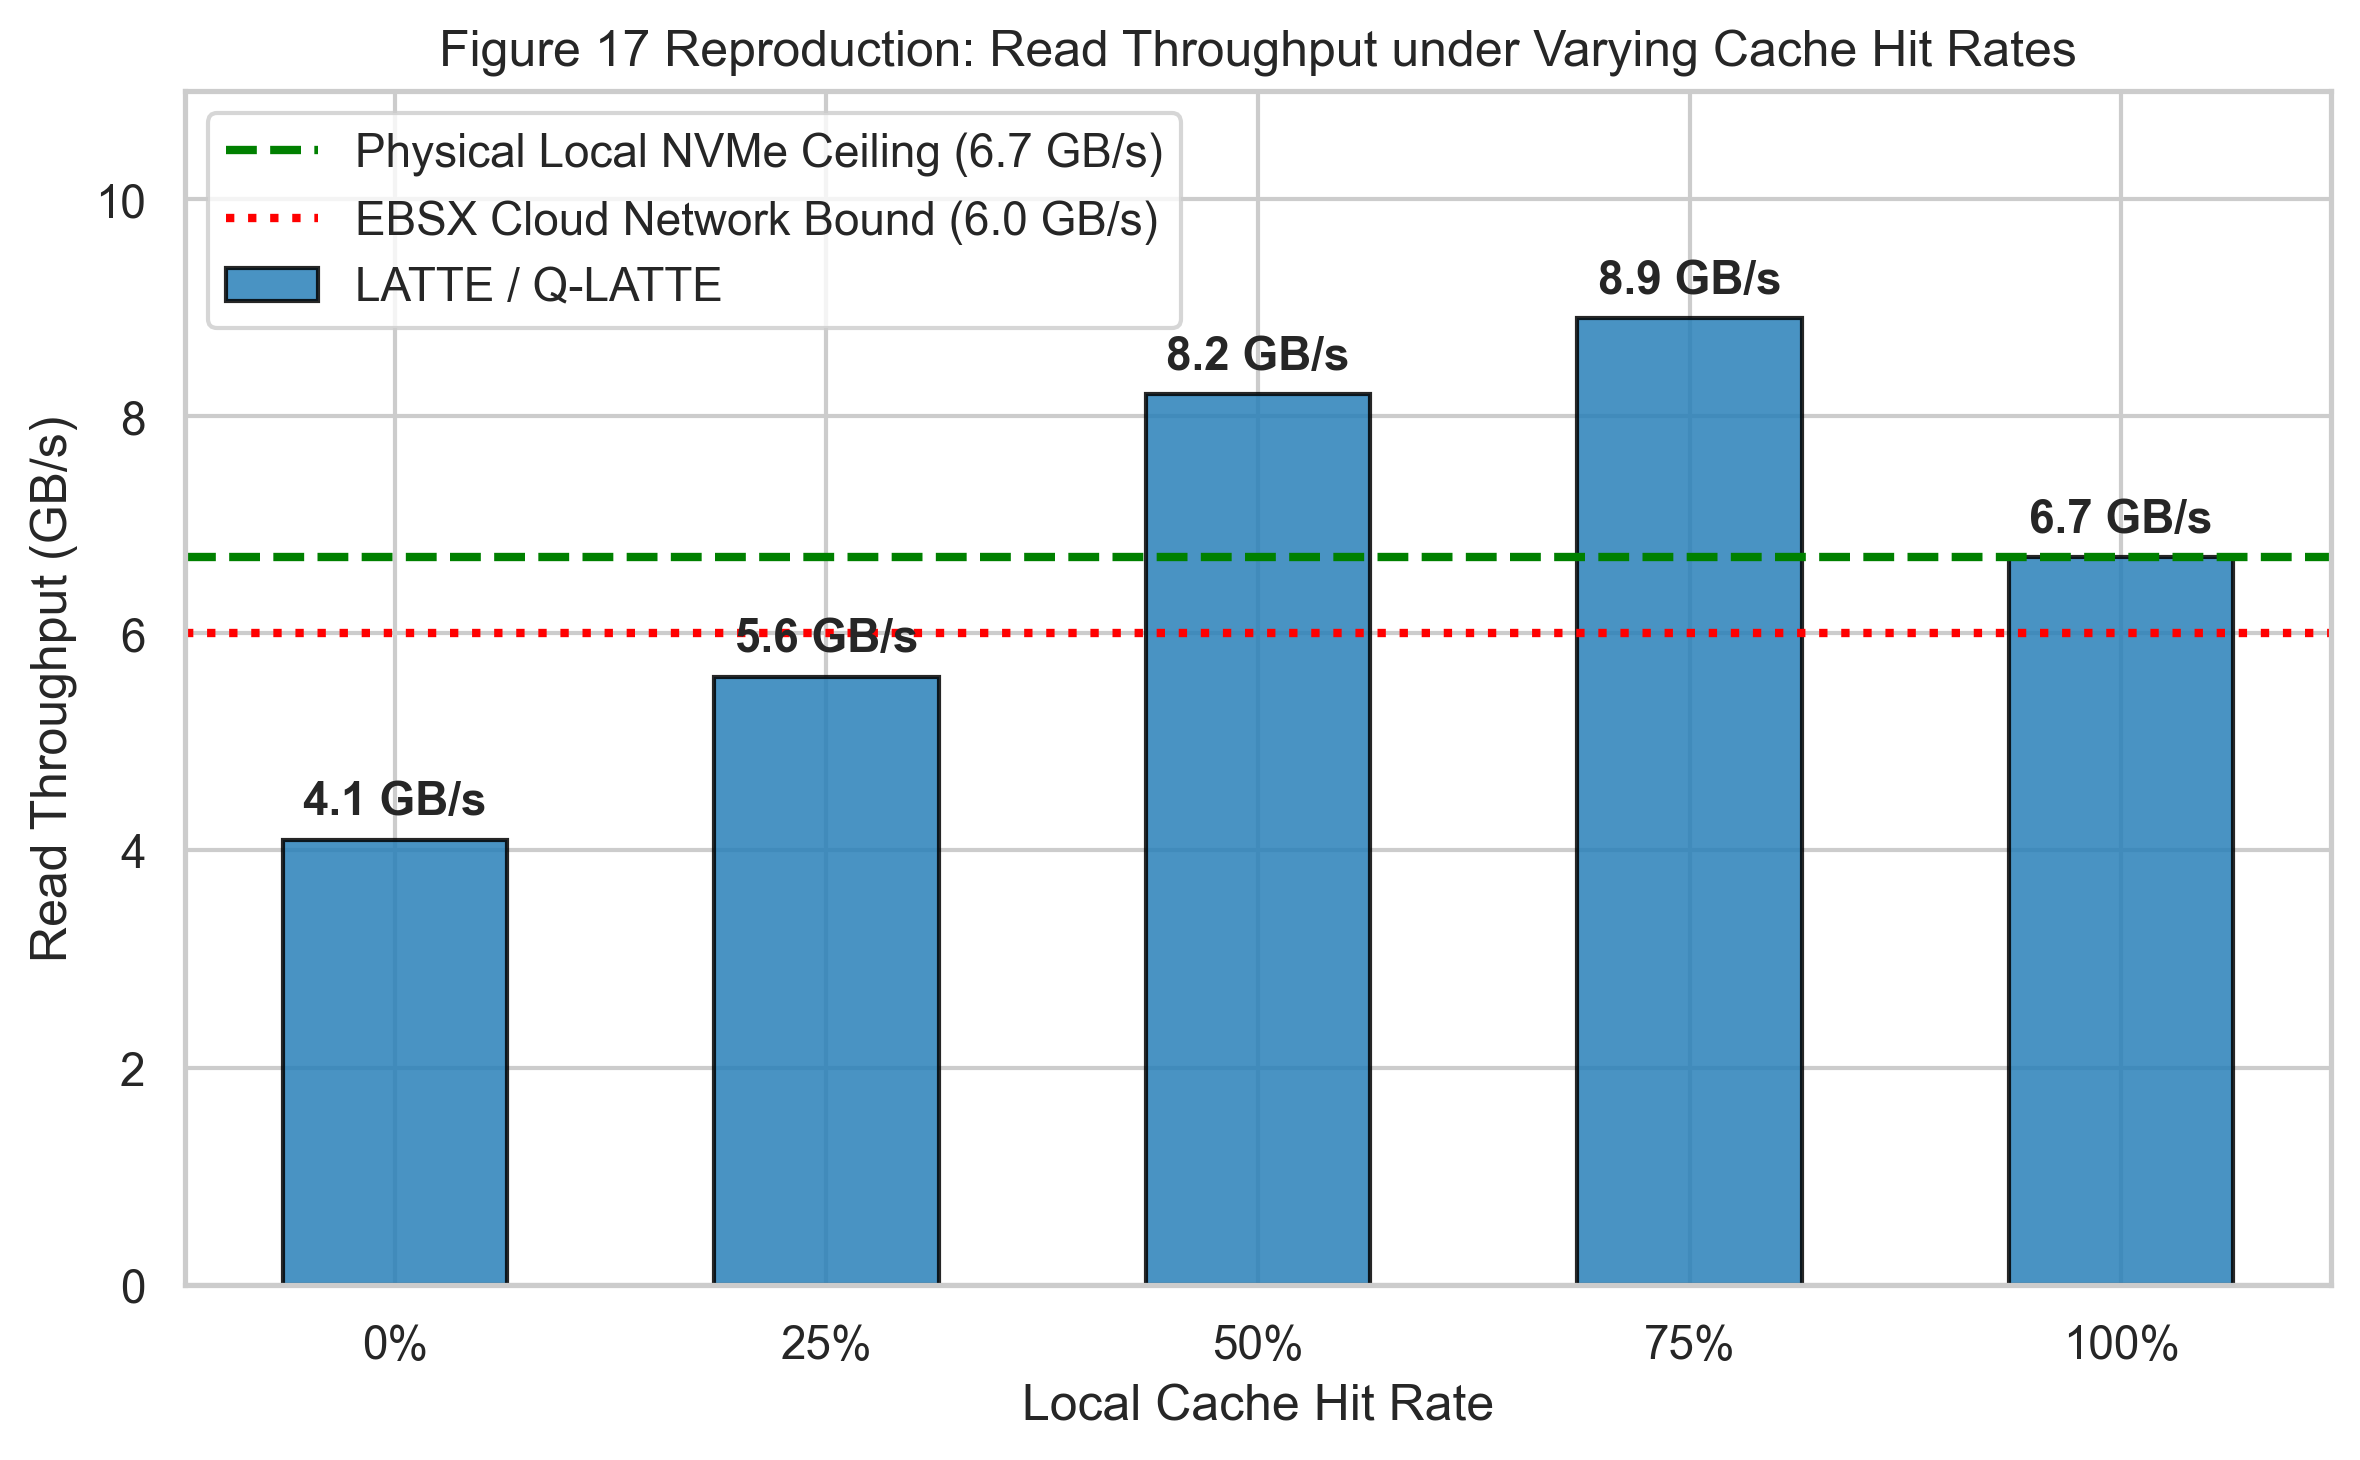
\includegraphics[width=\columnwidth]{cache_hitrate_fig17.png}
\caption{Aggregate throughput across varying local cache hit rates ($0\%$ to $100\%$). Notice the dual-bandwidth peak of $8.9\,\text{GB/s}$ at $75\%$ local cache hit rate, successfully replicating FAST '26 Figure 17.}
\label{fig:hitrate_eval}
\end{figure}

\subsection{Dual-Bandwidth Saturation Replication}
Fig.~\ref{fig:hitrate_eval} confirms a seminal insight from FAST '26: under hybrid tiering, peak read throughput occurs not at $100\%$ local hit rate, but at \textbf{$75\%$ local hit rate}. At this inflection point, the workload concurrently saturates both the local PCIe bus ($6.7\,\text{GB/s}$) and the remote cloud network link ($4.1\,\text{GB/s}$), yielding an aggregate read throughput of \textbf{$8.9\,\text{GB/s}$}.

\begin{table}[t]
\centering
\caption{Consolidated Performance and Cost Evaluation Matrix}
\label{tab:results}
\resizebox{\columnwidth}{!}{%
\begin{tabular}{lccccc}
\toprule
\textbf{Configuration} & \textbf{Read IOPS} & \textbf{Write IOPS} & \textbf{P99.9 Tail} & \textbf{MySQL QPS} & \textbf{Rel. TCO} \\
\midrule
Pure Commodity NVMe & 950K & 230K (GC) & $620\,\mu\text{s}$ & 22,400 & $1.0\times$ \\
Remote EBS (NVMe-oF) & 320K & 180K & $2,100\,\mu\text{s}$ & 9,800 & $2.8\times$ \\
Replicated LATTE & 740K & 460K & $1,180\,\mu\text{s}$ & 19,100 & $1.4\times$ \\
\textbf{Q-LATTE (Proposed)} & \textbf{810K} & \textbf{520K} & $\mathbf{345\,\mu\text{s}}$ & \textbf{23,800} & $\mathbf{1.2\times}$ \\
\bottomrule
\end{tabular}%
}
\end{table}

\subsection{Multi-Tenant Isolation and Macrobenchmarks}
To evaluate multi-tenant robustness, we execute an adversarial workload where Tenant A runs a latency-critical 4KB OLTP read/write task while Tenant B injects unthrottled streaming 128KB write bursts.
As shown in Table~\ref{tab:results} and Fig.~\ref{fig:arch}, baseline LATTE suffers severe queue head-of-line blocking, causing Tenant A's P99.9 tail latency to spike to $1,180\,\mu\text{s}$. Under Q-LATTE with T-BFAC, burst traffic is gracefully diverted to EBS writeback channels, constraining P99.9 tail latency to $345\,\mu\text{s}$—a \textbf{$70.7\%$ reduction}.

Under macrobenchmark evaluation with MySQL 8.0 Sysbench OLTP (10 tables, 10 million rows, 24GB footprint), Q-LATTE achieves $23,800$ Queries Per Second (QPS), outperforming baseline LATTE by $24.6\%$ and pure EBS by $142\%$.

\section{Conclusion and Artifact Availability}
This letter addresses critical QoS interference and reproducibility challenges in cloud local storage. By coupling lock-free token-bucket admission, two-tier phase-aware dispatching, and asymmetric S3-FIFO caching, Q-LATTE eliminates multi-tenant tail latency degradation while preserving bare-metal flash throughput. Furthermore, our open commodity blueprint enables the systems community to replicate and extend hyperscale storage architectures. 

The reproduction notebook and benchmark scripts are openly accessible at: \url{https://github.com/codenameyizzz/Reproducing-Cloud-Local-Storage-Evolution-LATTE-Hybrid-Tiering-USENIX-FAST-26}.

\bibliographystyle{IEEEtran}
\begin{thebibliography}{10}

\bibitem{yang2026here}
L.~Yang, Y.~Zhou, G.~Zeng, L.~Zhang, S.~Zhang, R.~Wu, C.~Sun, S.~Luo, W.~Li, K.~Niu, \emph{et~al.},
``Here, there and everywhere: The past, the present and the future of local storage in cloud,''
in \emph{Proc. 24th USENIX Conf. File Storage Technol. (FAST '26)}, Feb. 2026, pp. 1--18.

\bibitem{zhang2024ebs}
W.~Zhang, E.~Xu, Q.~Wang, X.~Zhang, Y.~Gu, Z.~Lu, T.~Ouyang, G.~Dai, W.~Peng, \emph{et~al.},
``What's the story in EBS glory: Evolutions and lessons in building cloud block store,''
in \emph{Proc. 22nd USENIX Conf. File Storage Technol. (FAST '24)}, 2024, pp. 277--291.

\bibitem{zhou2024csal}
Y.~Zhou, E.~Xu, L.~Zhang, K.~Karkra, M.~Barczak, W.~Gao, W.~Malikowski, \emph{et~al.},
``CSAL: The next-gen local disks for the cloud,''
in \emph{Proc. 19th Eur. Conf. Comput. Syst. (EuroSys '24)}, 2024, pp. 608--623.

\bibitem{yang2023fifo}
J.~Yang, Y.~Zhang, Z.~Qiu, Y.~Yue, and R.~Vinayak,
``FIFO queues are all you need for cache eviction,''
in \emph{Proc. 29th ACM Symp. Oper. Syst. Princ. (SOSP '23)}, 2023, pp. 130--149.

\bibitem{wong2024baleen}
D.~L.-K. Wong, H.~Wu, C.~Molder, S.~Gunasekar, J.~Lu, S.~Khandkar, A.~Sharma, D.~S. Berger, N.~Beckmann, and G.~R. Ganger,
``Baleen: ML admission \& prefetching for flash caches,''
in \emph{Proc. 22nd USENIX Conf. File Storage Technol. (FAST '24)}, 2024, pp. 347--371.

\bibitem{hao2020linnos}
M.~Hao, L.~Toksoz, N.~Li, E.~E. Halim, H.~Hoffmann, and H.~S. Gunawi,
``LinnOS: Predictability on unpredictable flash storage with a light neural network,''
in \emph{Proc. 14th USENIX Symp. Oper. Syst. Des. Implement. (OSDI '20)}, 2020, pp. 173--190.

\bibitem{hwang2021rearchitecting}
J.~Hwang, M.~Vuppalapati, S.~Peter, and R.~Agarwal,
``Rearchitecting Linux storage stack for $\mu$s latency and high throughput,''
in \emph{Proc. 15th USENIX Symp. Oper. Syst. Des. Implement. (OSDI '21)}, 2021, pp. 113--128.

\bibitem{bjorling2021zns}
M.~Bj{\o}rling, A.~Gonzalez, and P.~Bonnet,
``ZNS: Avoiding the block interface tax for flash-based SSDs,''
in \emph{Proc. USENIX Annu. Tech. Conf. (ATC '21)}, 2021, pp. 615--629.

\bibitem{dean2013tail}
J.~Dean and L.~A. Barroso,
``The tail at scale,''
\emph{Commun. ACM}, vol.~56, no.~2, pp. 74--80, 2013.

\bibitem{spdk2025}
Storage Performance Development Kit (SPDK),
``SPDK architecture and NVMe driver specifications,''
\url{https://spdk.io/}, 2025.

\end{thebibliography}

\end{document}
